\chapter{Este es el primer capítulo}

\section{Ecuaciones}

\subsection{Ecuaciones de escalares}

Letras mayúsculas para constantes ($A$, $T$, $L_a$), minúsculas para variables ($x$, $y$, $v_a$).

\begin{equation}
	\dot {\hat x} = A \hat x + B u + L \left( y - C \hat x \right)  
\end{equation}


\subsection{Ecuaciones con matrices}

Letras mayúsculas para matrices de constantes ($\mathbf{A}$, $\mathbf{T}$, $\mathbf{L}_a$), minúsculas para variables ($\mathbf{x}$, $\mathbf{y}$, $\mathbf{v}_a$).

\begin{equation}
	\mathbf{\dot {\hat  x} = A \hat x + B u + L \left( y - C \hat x \right) }
\end{equation}

\subsection{Ecuaciones de fasores o complejos}

\begin{equation}
	\underline S_1 = \sqrt{3} \underline U_1 \overline{\underline I_1} 
\end{equation}

\section{Tablas}

\subsection{Tablas sin entorno}


\begin{tabular}{lcc}
\toprule
Tecnología & Potencia & Porcentaje \\ 
\midrule
Ciclo  & 15 & $20\%$ \\ 
Eólica & 22 & $25\%$ \\ 
Nuclear & 7 & $25\%$ \\ 
Hidráulica & 10 & $25\%$ \\ 
\bottomrule
\end{tabular} 

\subsection{Tablas con entorno}

\begin{table}
\centering
\begin{tabular}{lcc}
\toprule
Tecnología & Potencia & Porcentaje \\ 
\midrule
Ciclo  & 15 & $20\%$ \\ 
Eólica & 22 & $25\%$ \\ 
Nuclear & 7 & $25\%$ \\ 
Hidráulica & 10 & $25\%$ \\ 
\bottomrule
\end{tabular} 

\caption{Tabla con entorno}
\label{tbl:nombre_tabla}
\end{table}


 
\begin{figure}
	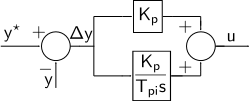
\includegraphics[width=\textwidth]{model/pdf/pi.pdf} 
	\caption{Control proporcional integral}
	\label{ctrl_pi}
\end{figure}
 
 
\begin{figure}
	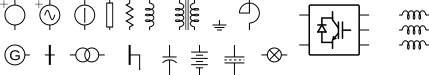
\includegraphics[width=\textwidth]{./pdf/circuitos.pdf} 
	\caption{Libreria de circuitos (ver .svg con inkscape)}
	\label{fig:circuitos}
\end{figure}

 \cite{Rodriguez2007}
 
 
 
 

